\documentclass{bioinfo}
\copyrightyear{2017}
\pubyear{2017}

% amsmath package, useful for mathematical formulas
\usepackage{amsmath}
% amssymb package, useful for mathematical symbols
\usepackage{amssymb}

\usepackage{graphicx}
\usepackage{subfigure}
% cite package, to clean up citations in the main text. Do not remove.
\usepackage{cite}

\usepackage{url}

\begin{document}
\firstpage{1}

% Title must be 150 characters or less
\title[Tracer 1.6]{Bayesian MCMC diagnostics and summarisation using Tracer 1.6}

\author[Rambaut \textit{et~al}]{ Andrew Rambaut\,$^{1}$, Alexei J.~Drummond\,$^{2,3}$, Dong Xie\,$^{2,3}$, Marc A.~Suchard\,$^{4,5}$}

\address{
$^{1}$Institute of Evolutionary Biology, University of Edinburgh, Edinburgh, UK\\
$^{2}$Department of Computer Science, University of Auckland, Auckland, NZ\\
$^{3}$Centre for Computational Evolution, University of Auckland, Auckland, NZ\\
$^{4}$Departments of Biomathematics and Human Genetics, David Geffen School of Medicine, UCLA, and \\
$^{5}$Department of Biostatistics, UCLA Fielding School of Public Health, University of California, Los Angeles, USA \\
}

\history{Received on XXXXX; revised on XXXXX; accepted on XXXXX}

\editor{Associate Editor: XXXXXXX}

\maketitle


% Please keep the abstract between 250 and 300 words
\begin{abstract}

\section{Motivation:}
%Computational evolutionary biology, statistical phylogenetics and coalescent-based population genetics are becoming increasingly central to the analysis and understanding of molecular sequence data.
Bayesian inference of phylogeny using Markov chain Monte Carlo (MCMC) plays a central role in understanding evolutionary history and processes from molecular sequence data.
Visualising and analysing the samples from the posterior distribution is a key step in any non-trivial Bayesian inference, and it is especially important for methods that employ MCMC.
\section{Results:}
Here we present a software package \emph{Tracer} (version 1.6) for visualising and analysing the trace files generated by Bayesian MCMC runs.
The \emph{Tracer} software also provides kernel density estimation, cheap marginal likelihood estimation,
multivariate visualisation, demographic trajectory reconstruction, conditional posterior distribution summary and more.
\section{Availability:}
Tracer is open-source under the GNU lesser general public license and available at
\url{http://beast.bio.ed.ac.uk/Tracer} and \url{https://github.com/beast-dev/tracer}.

\section{Contact:}
\href{a.rambaut@ed.ac.uk}{\url{a.rambaut@ed.ac.uk}},
\href{alexei@cs.auckland.ac.nz}{\url{alexei@cs.auckland.ac.nz}}
and
\href{msuchard@ucla.edu}{\url{msuchard@ucla.edu}}

\end{abstract}

\section*{Introduction}

Bayesian inference of phylogeny using Markov chain Monte Carlo (MCMC) \citep{rannala1996probability,mau1999bayesian} flourishes as a popular approach to uncover the evolutionary relationships among taxa, whether genes, genomes, individuals or species.
MCMC approaches generate samples of model parameter values including the phylogenetic tree drawn from their posterior distribution given molecular sequence data.
Visualising, tabulating and marginalising these samples is critical for approximating the posterior quantities of interest that one reports in a Bayesian phylogenetic analysis.
%However, the full posterior distribution is high-dimensional and often difficult to visualise.
To facilitate this task, we develop the Tracer (version 1.6) software package that parses MCMC log files of samples to interactively explore the high-dimensional posterior distribution.
%
%containing the list of parameters whose values sampled from the chain.
Tracer works automatically with sample output from
%It can be used to analyse runs of
BEAST 1 \citep{drummond2012bayesian}, BEAST 2 \citep{bouckaert2014beast2}, MrBayes \citep{ronquist2012mrbayes}, RevBayes \citep{hohna2016revbayes}, LAMARC \citep{kuhner2006lamarc}, Migrate \citep{beerli2006comparison} and possibly other MCMC programs from other domains.

(move to somewhere else) In addition, Tracer's demographic reconstruction functions are utilised to redraw the distribution of effective population sizes over time if an available demographic model was involved in the analysis.


%\begin{itemize}
%\item Importance of posterior summaries (as scientifically relevant marginalization of the full posterior distribution)
%\item Full posterior distribution is high-dimensional and (often) difficult to visualize
%\item Posterior simulator agnostic -- highly used with \textsc{MrBayes} as well
%\end{itemize}

\section*{Design and Implementation}

\begin{figure}[ht]
\centerline{
\includegraphics[width=0.45\textwidth]{./figures/tracer.pdf}
}
\caption{The system design of Tracer 1.6}
\label{fig:tracer}
\end{figure}

Tracer is able to analyse either a single MCMC log or combine the shared traces from multiple logs as designed in Figure~\ref{fig:tracer}.
The list of traces in each log are created from the sampling parameters logged during a MCMC process, which include their statistical summaries from their values at all states logged.
The effective sample size (ESS) is an important measurement designed for a sampled parameter having continuous values, which tells the number of effectively independent draws from the posterior distribution that the Markov chain is equivalent to.

Tracer handles three trace types, also known as variable types \citep{mendenhall2012introduction}: real, integer, and categorical.
The real trace is used to handle quantitative continuous variables, which is the most common type in logged parameters.
The integer is dealing with quantitative discrete variables, and the categorical trace is for qualitative categorical variables.
% check above definition
%These three types can be automatically assigned when the log file is imported. But they can also be changed later.

The multiple traces can be selected as shown in Figure~\ref{fig:multitrace}, which will overlay the plots for the different traces allowing comparisons to be made. The multiple trace files can be similarly selected as well to compare different runs. If multiple trace files have the same trace names,  then a ``Combined'' trace will automatically appear, which can be selected as well as the individual trace files.

\begin{figure}[ht]
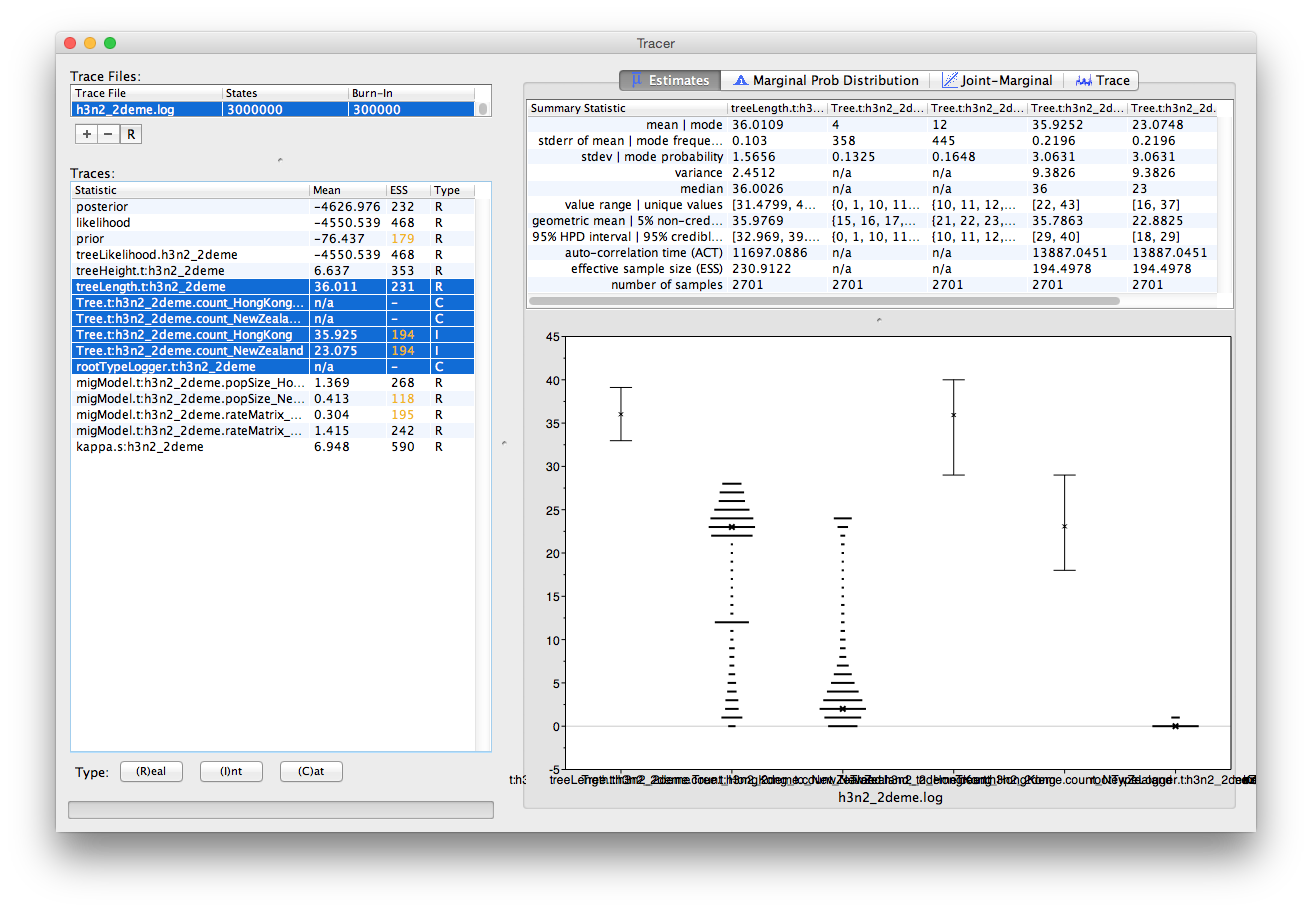
\includegraphics[width=.5\textwidth]{./figures/multitrace.png}
\caption{A comparison of multiple traces}
\label{fig:multitrace}
\end{figure}

There are four analysis tabs to choose from either a selected trace (sampling parameter) or multiple traces:

%TODO simplify, some duplication to 1st example
\begin{itemize}
\item Estimates - this shows the mean, standard deviation, confidence intervals, ESS, and other statistics about the selected trace(s). A histogram presenting the frequency distribution over values will also be plotted for a single selected trace, such as Figure~\ref{fig:4tabs}.a. Interval bars for quantitative traces (real or integer) or violin plots for categorical traces will be drawn for a comparison, such as Figure~\ref{fig:multitrace}, if multiple traces are selected.

\item Density - this shows the Bayesian posterior density plot for the selected trace(s), if they are continuous, the kernel density estimates will be available for continuous traces, for example, in Figure~\ref{fig:4tabs}.b.

\item Joint-Marginal - this only appears if exactly two traces are chosen. It then plots one against the other to look at their joint-marginal distribution, for example, in Figure~\ref{fig:4tabs}.c.

% trace is duplicate to trace, use trajectory?
\item Trace - this shows the trajectory of the selected trace(s) against state or generation number as it can be seen in Figure~\ref{fig:4tabs}.d. It can be used to check mixing, choose a suitable burn-in and look for trends that might suggest problems with convergence.

\end{itemize}

In addition to illustrating joint-marginal distribution between two continuous traces, we newly invented a TangHuLu chart to visualise the joint probability between two integer or categorical traces using coloured bubbles, as shown in Figure~\ref{fig:tanghulu}.a. The size of circle is proportional to the joint probability, the blue coloured circle is in the credible set of given a probability threshold default to 0.95, the red is in the set not in the credible set. The tile background is coloured if there is any circle, in case the very small circle wouldn't be missed out. The coloured background can also help to show the area of the credible set and non-credible set.

Furthermore, box-and-whisker plots are used to display the joint-marginal distribution between one continuous trace and one integer or categorical trace as shown in Figure~\ref{fig:tanghulu}.b.

\begin{figure}[ht]
\subfigure[TangHuLu chart]{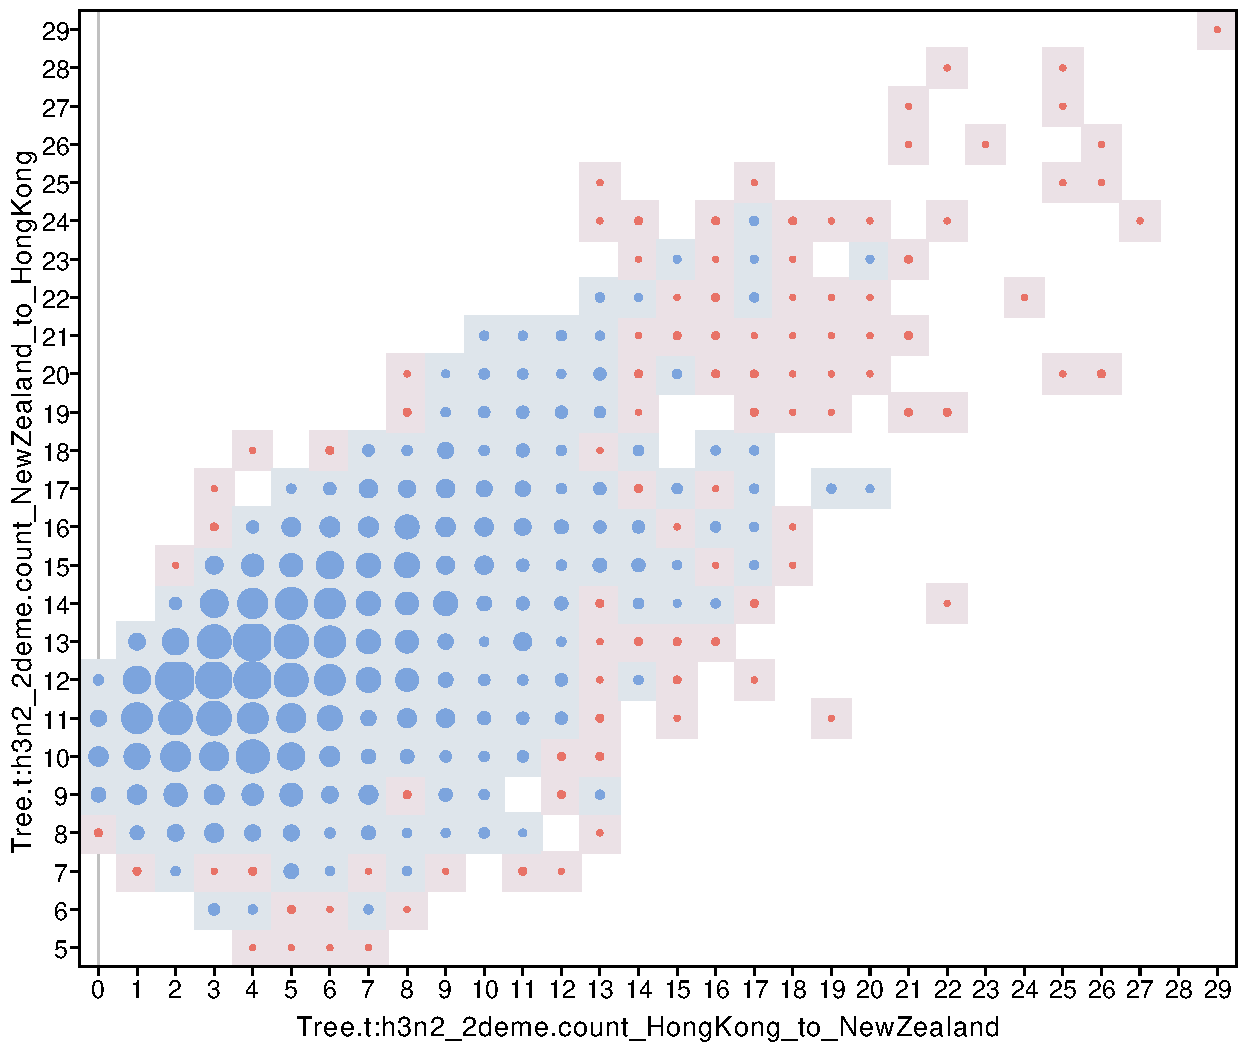
\includegraphics[width = .23\textwidth, height = 3cm]{./figures/tanghulu.pdf}}
\subfigure[boxplot]{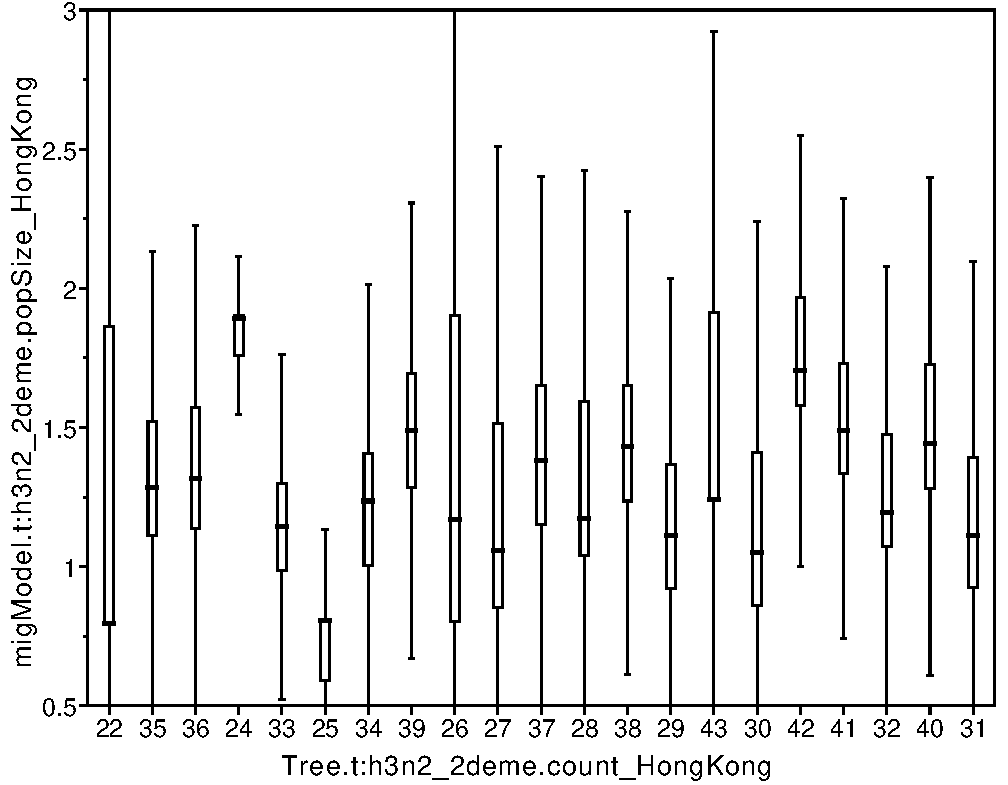
\includegraphics[width = .23\textwidth, height = 3cm]{./figures/boxplot.pdf}}
\caption{Visualisation of joint-marginal distribution (a) between two integer or categorical traces using TangHuLu chart, and (b) between one continuous trace and one integer or categorical trace using box-and-whisker plot.}
\label{fig:tanghulu}
\end{figure}

A key feature of Tracer lies in its ability to link together samples from quantitative random variable log files and tree log files.
This linkage is not available in other popular post-processing MCMC software, such as coda \citep{plummer2006coda} and AWTY \citep{nylander2007awty}, and enables users to approximate the posterior distribution of scientifically relevant quantities that are functions of both the tree and other quantitative measures.
Demographic reconstruction through time is a prime example.


Tracer also provides demographic reconstruction resulting in a graphical plot, often applyed to reconstruct epidemic dynamics, given a MCMC log from a Bayesian framework or additionally with the tree log depending on the model.
The currently available models are constant size \citep{drummond2002estimating}, exponential growth \citep{drummond2002estimating}, logistic growth (?), Bayesian coalescent skyline \citep{drummond2005bayesian}, GMRF Bayesian skyride \citep{minin2008smooth}, and Bayesian coalescent skygrid \citep{gill2012improving}.
%For example, ``Demographic Reconstruction" performs reconstructions of the distribution for a number of models, such as constant size \citep{drummond2002estimating}, exponential growth \citep{drummond2002estimating}, and logistic growth (?). %citation?
%Besides ``Bayesian Skyline Reconstruction'' reconstructs a generalised Bayesian coalescent skyline plot (e.g. Figure~\ref{fig:flu}.a) describing demographic history under canonical scenarios \citep{drummond2005bayesian},
%``GMRF Skyride Reconstruction'' and ``SkyGrid Reconstruction'' are respectively available for a temporal smoothing method using the Gaussian Markov random field (GMRF) model  \citep{minin2008smooth} and a generalisation of the GMRF model \citep{gill2012improving}.
Besides these, ``Lineages Through Time'' (?) is also available to plot the quantiles of the number of lineages against time, which describes the change of diversification of all organisms over time. %citation?
%All these models are available in BEAST \citep{drummond2007beast}.

%TODO is it OK ?
Tracer recently offers a fairly general solution of looking at conditional posterior distributions. This, specifically, supports for Bayesian stochastic search variable selection (BSSVS) forms of model averaging, in which some parameters are only in the likelihood when their sub-model is indicated by an indicator function usually assigned to a discrete, integer or boolean variable. In that case, the posterior of the parameter should not include the states when it was sampled only in the prior, because the sub-model it belonged to was ``turned off". This is relevant for extended Bayesian skyline plot, random local clock model, microsatellite model averaging, and relaxed clock model averaging methods, etc. It is also relevant for BSSVS in phylogeography as well depending on how the state is logged.

% TODO more ?

\section*{Example}

%Even users of \textsc{MrBayes} and \textsc{RevBayes} find Tracer handy.

\subsection*{Calibrating the tree to estimate TMRCA}

Figure~\ref{fig:4tabs} demonstrates a snapshot of posterior summaries in Tracer for a BEAST \citep{drummond2012bayesian} run created from a 898 bp alignment of sequences of 12 species of primates (http://beast.bio.ed.ac.uk/tutorials?). %data citation

%using HKY + $\Gamma_4$ model, uncorrelated lognormal relaxed molecular clock, and Yule prior on the tree.
In this analysis, we furthermore specified three calibrations on the phylogenetic tree to estimate time to the most recent common ancestor (TMRCA) based on our prior fossil knowledge.

The first TMRCA prior, called ``ingroup'', includes all species except the \textit{Lemur} which will form the outgroup in the tree. %monophyletic
The second group is ``Human-Chimp'' that contains only \textit{Homo sapiens} and \textit{Pan}.
The last consists of everything except \textit{Lemur}, \textit{Saimiri} and \textit{Tarsius} to create the hominoid-cercopithecoid split, which is named as ``HomiCerco''.
We know the most recent common ancestor of humans and chimps may live about $5-7$ million years ago, a normal distribution centered at 6 million years with a standard deviation of 0.5 million years is assigned to the ``Human-Chimp'' prior.
Another normal distribution of $24 \pm 0.5$ (million years) is likewise defined for ``HomiCerco''.

\begin{figure}[ht]
\subfigure[Estimates]{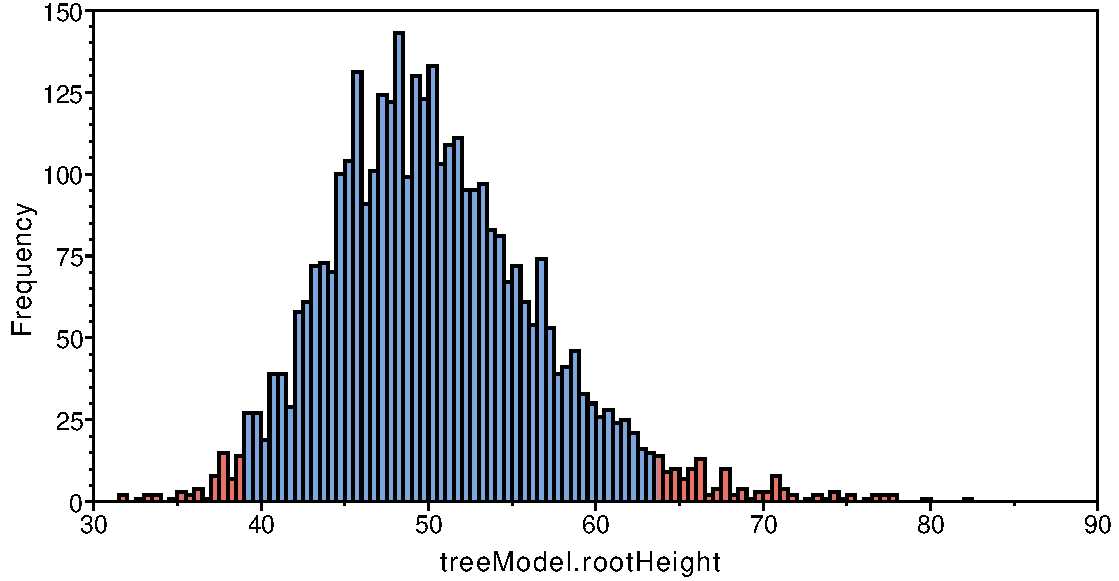
\includegraphics[width = .23\textwidth, height = 3cm]{./figures/treeRootHeight.pdf}}
\subfigure[Density]{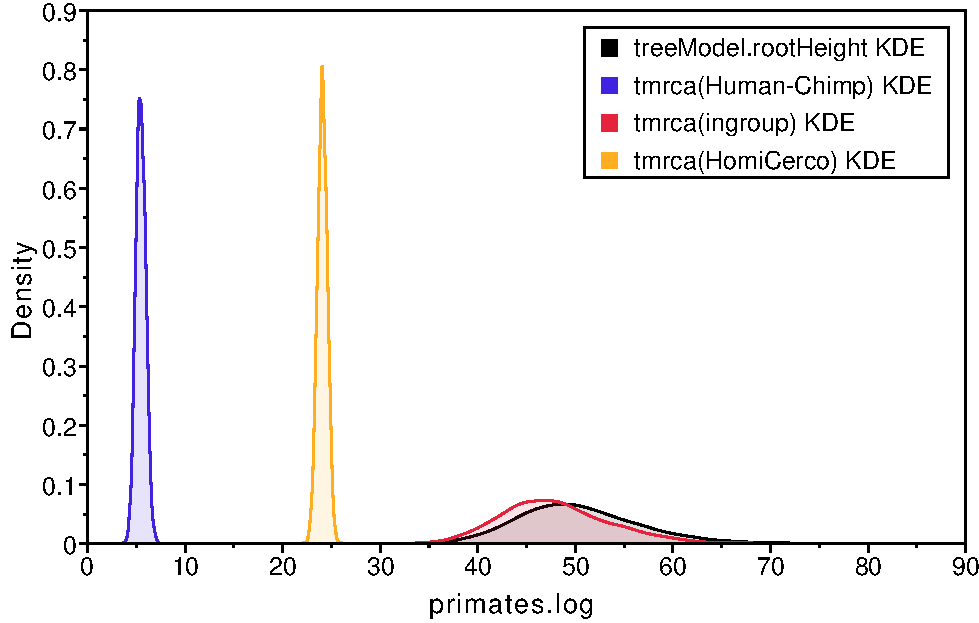
\includegraphics[width = .23\textwidth, height = 3cm]{./figures/multiKDE.pdf}}\\
\subfigure[Joint-Marginal]{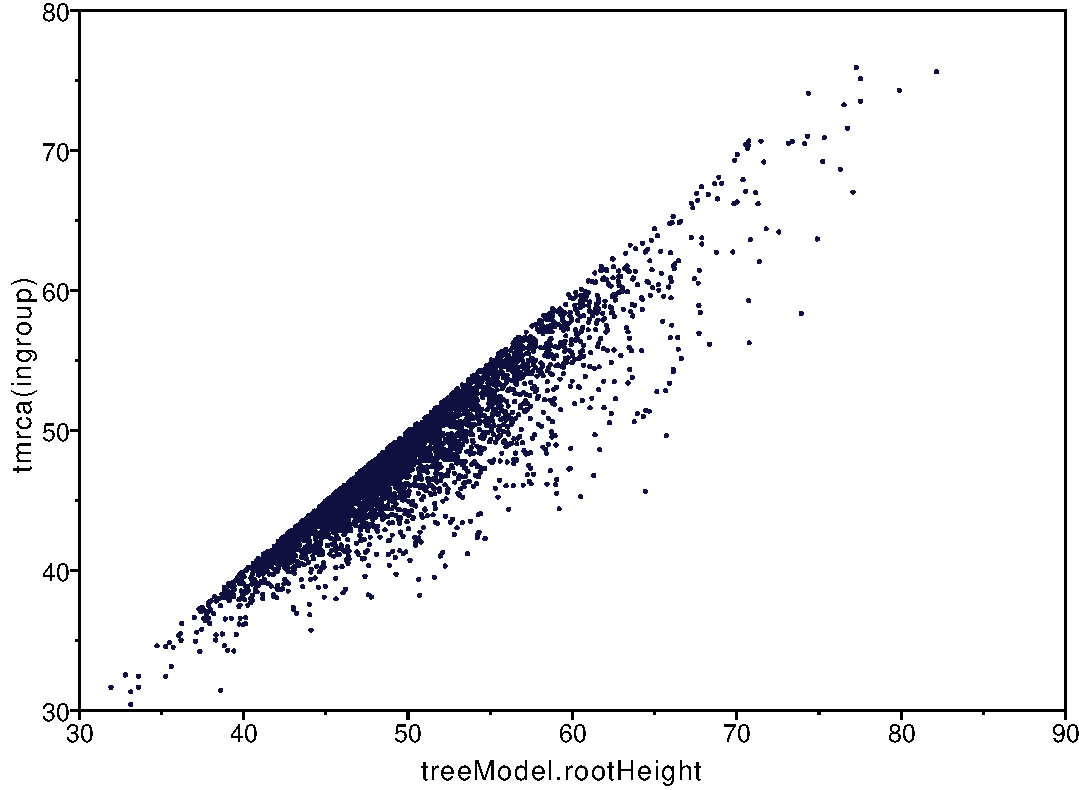
\includegraphics[width = .23\textwidth, height = 3cm]{./figures/joint-marginal-th-ingroup.pdf}}
\subfigure[Trace]{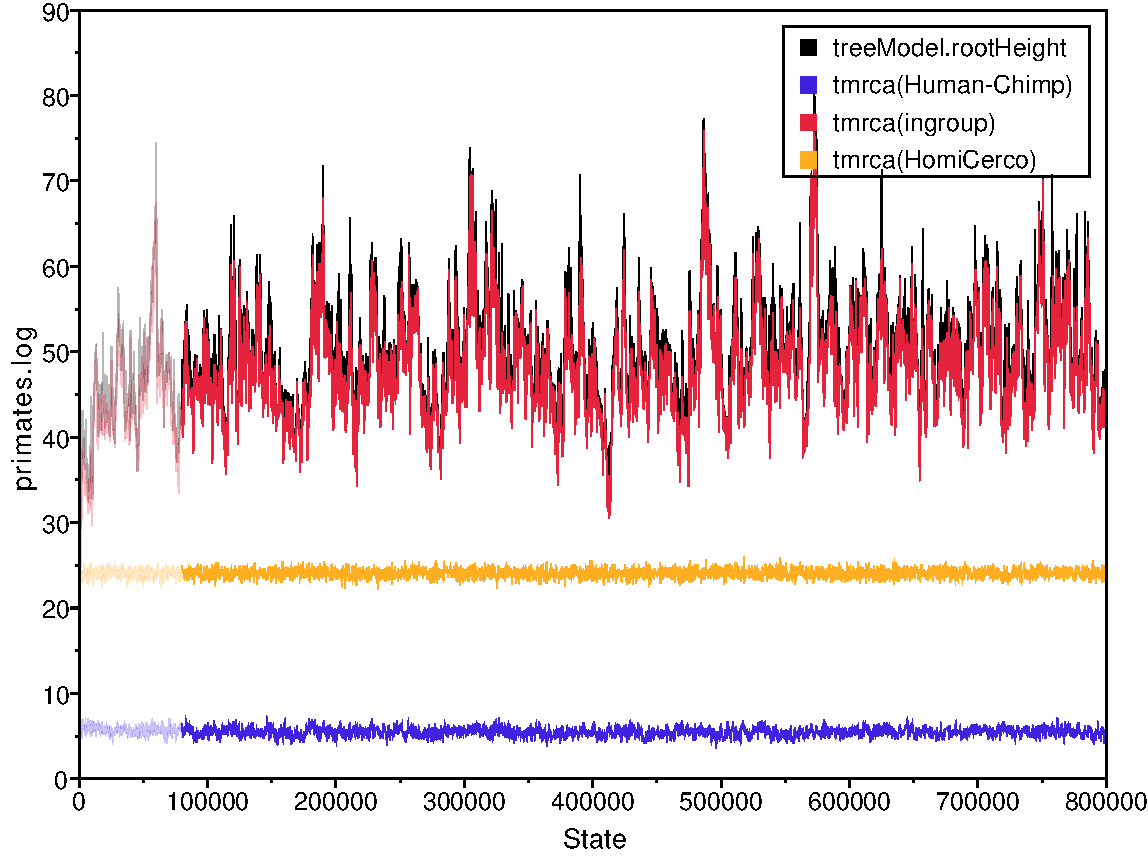
\includegraphics[width = .23\textwidth, height = 3cm]{./figures/trace.pdf}}
\caption{Images exported from four analysis tabs in Tracer for calibrating the tree to estimate TMRCA, where the black is ``treeModel.rootHeight'' parameter, blue is TMRCA parameter of ``Human-Chimp'', red is ``ingroup'', and yellow is ``HomiCerco''.}
\label{fig:4tabs}
\end{figure}

After loading the log, selecting the ``treeModel.rootHeight'' parameter gives the marginal posterior distribution of the age of the root of entire tree. The blue bars in Figure~\ref{fig:4tabs}.a present the most compact interval on the root height of the tree that contains 95\% of the posterior probability, referring to the period between about 39.01 and 63.67 million years old with the mean of 50.48 million years.
%TODO rate is faster than Yang's book r_ape = 5.4 * 10^-10 per year, r_monkey = 8.0, r_root = 6.6
Correspondingly selecting ``meanRate'' provides the rate of evolution averaged over the whole tree, which has the mean of 0.0129 substitutions per site per million years with 95\% HPD Interval between 0.0101 and 0.0159.

Figure~\ref{fig:4tabs}.b shows the kernel density estimations of these four parameters. The two TMRCA parameters, ``Human-Chimp'' in blue and ``HomiCerco'' in yellow, that we used to calibrate the tree explicitly have posterior distributions very similar to the prior distributions that we specified.

The marginal posterior densities of ``treeModel.rootHeight'' and ``ingroup'' are nearly overlapped each other. When we switch to their joint-marginal distribution plot in Figure~\ref{fig:4tabs}.c, the samples are almost lined up together, which indicates they are associated.
But this isn't an issue here, because the ``ingroup'' only excludes one outgroup species from all taxa.
%TODO how to explain this problem further?

Figure~\ref{fig:4tabs}.d illustrates the traces of these four parameters against their logged states from MCMC chain. ``Human-Chimp'' and ``HomiCerco'' parameters are immediately reaching equilibrium from the starting point, but ``treeModel.rootHeight'' and ``ingroup'' clearly show a burn-in period. %TODO ?

\subsection*{Non-parametric coalescent estimator}

In the second example, there are two analyses conducted using a H3N2 data set that is the subset of a comprehensive influenza A virus data set spanning several epidemic seasons in the New York state. The data contains a  ?bp alignment of 165 Hemagglutinin genes collected between about 1999 and 2004 \citep{rambaut2008genomic}, explicating H3N2 spreading during three epidemic seasons.

To be able to reconstruct Bayesian coalescent skygrid \citep{minin2008smooth} plot, we exploit Tracer to exact past population dynamics from both MCMC log and tree log produced by a BEAST \citep{drummond2012bayesian} run.
The HKY + $\Gamma_4$ model, strict molecular clock, and Bayesian skygrid tree prior was respectively setup in the run, where a grid of 50 intervals over 5 years estimating 10 population sizes by year was constructed in the skygrid prior.

%What type of dynamics does the H3N2 skyride plot suggest?
According to Tracer's skygrid plot in Figure~\ref{fig:flu}.a, the changing patterns of genetic diversity in viral isolates from New York state clearly reveal the seasonal dynamics of influenza A in individual temperate populations. The absolute amount of genetic diversity, even at seasonal peaks, is small compared to other rapidly evolving viruses that infect far fewer people, suggesting that strong natural selection, in addition to periodic bottlenecks, reduces the level of diversity that co-circulates at any time. Simulations demonstrate that this reconstruction of genetic diversity is robust to the sampling protocol. %TODO copied from (Rambaut et al., 2008)


\begin{figure}[ht]
%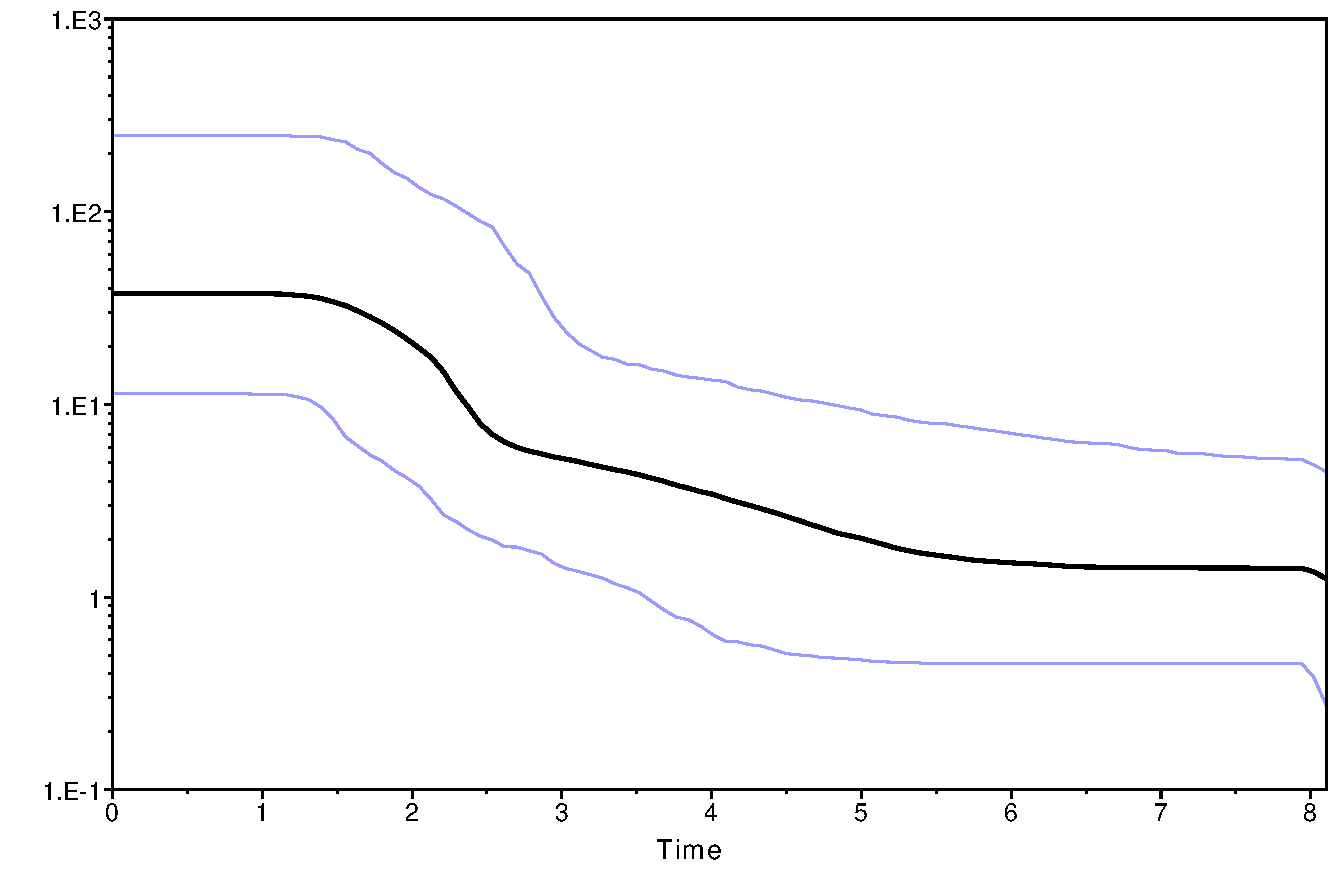
\includegraphics[width=.5\textwidth]{./figures/fluBSP.pdf}
\subfigure[Bayesian coalescent skygrid]{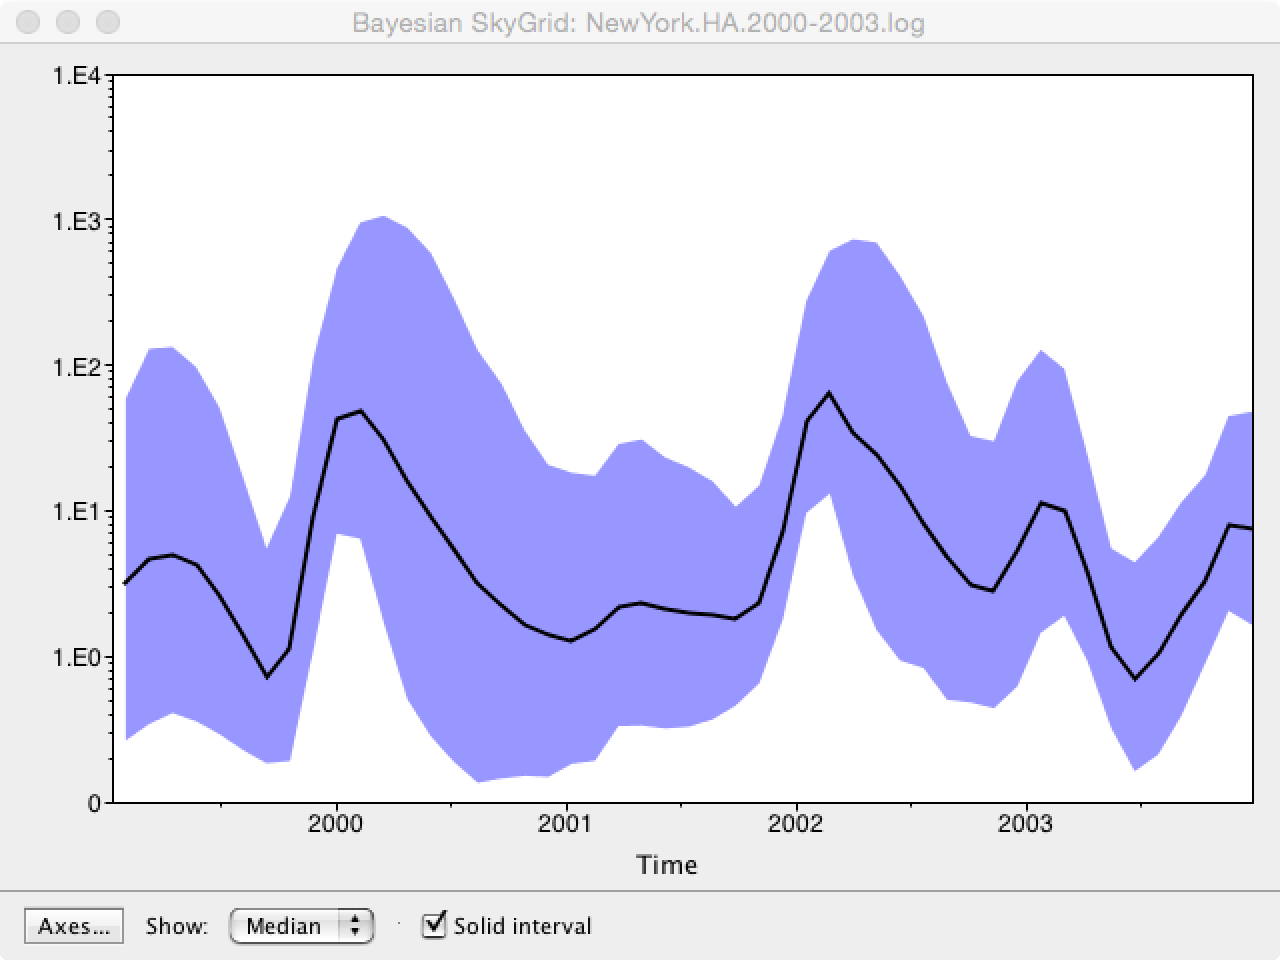
\includegraphics[width = .23\textwidth]{./figures/fig21.png}}
\subfigure[Lineages through time]{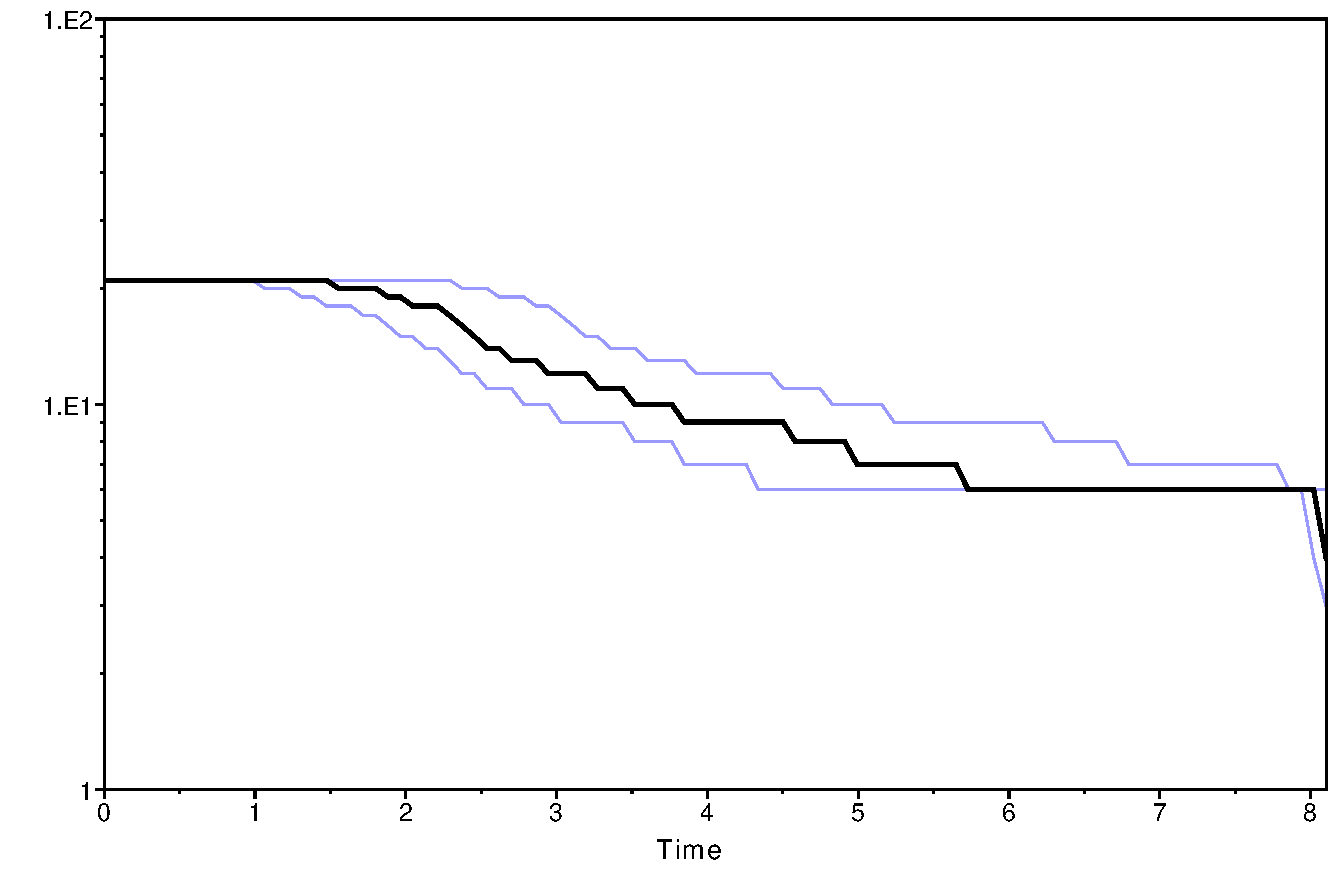
\includegraphics[width = .23\textwidth]{./figures/fluLTT.pdf}}
\caption{(a) Bayesian coalescent skygrid plot and (b) lineages through time for the Influenza A/H3N2 virus data.}
\label{fig:flu}
\end{figure}

Lineages Through Time in Figure~\ref{fig:flu}.b, similar curve

diversification has been gradually developed before 2003's break-out, but it also looks stopped after 2004.



\section*{Availability and Future Directions}

We make the Tracer package available in both executable and source code forms.  Tracer requires Java version 1.6 or greater and executables for Windows, Mac OS and Linux platforms are located at \url{http://beast.bio.ed.ac.uk/Tracer} % \url{https://github.com/beast-dev/tracer} ?
which serves as the main page for the package. This page also links to a sizeable list of self-contained, step-by-step tutorials covering basic to advance usage of Tracer to summarise posterior distributions of a large set of phylogenetic models simulated using BEAST.  For example, popular tutorials describe how to use Tracer to generate marginal parameter summaries and infer population dynamics trajectories over time.

Github houses the Tracer's source code within \url{https://github.com/beast-dev/tracer} ,and links to a GoogleGroup discussion group related to Tracer,
which is the ``beast-users" group (\url{http://groups.google.com/group/beast-users}) with over 1,500 members.
%At the time of writing, forty-seven developers belong to the ``beast-dev" group that facilitates BEAST development across three continents.

Future development directions for Tracer focus on \ldots



%\section*{Old Text}
%
%%You can also select the "Demographic Analysis" from the Analysis menu - This plots the distribution of demographic population sizes over time for a number of models (constant size, exponential growth \& logistic growth) that are available in BEAST. This involves you selecting the traces for each parameter of the model. You should only select the model that was actually run under BEAST (e.g., if you ran an exponential growth model, you shouldn't plot the constant population size model).
%
%%The "Analysis" menu also contains options for performing Bayesian Skyline reconstructions and for calculating Bayes Factors between runs.
%
%Feature list:
%\begin{itemize}
%\item KDEs
%\item cheap marginal likelihood estimators
%\item demographic trajectory reconstruction
%\end{itemize}
%
%%Model selection HME and AICM have been removed
%New features:
%\begin{itemize}
%\item Three trace types: real, integer, string
%\item Kernel density estimates
%\item Conditional posterior distribution
%%\item HME
%%\item AICM
%\end{itemize}
%
%%\begin{figure}[H]
%%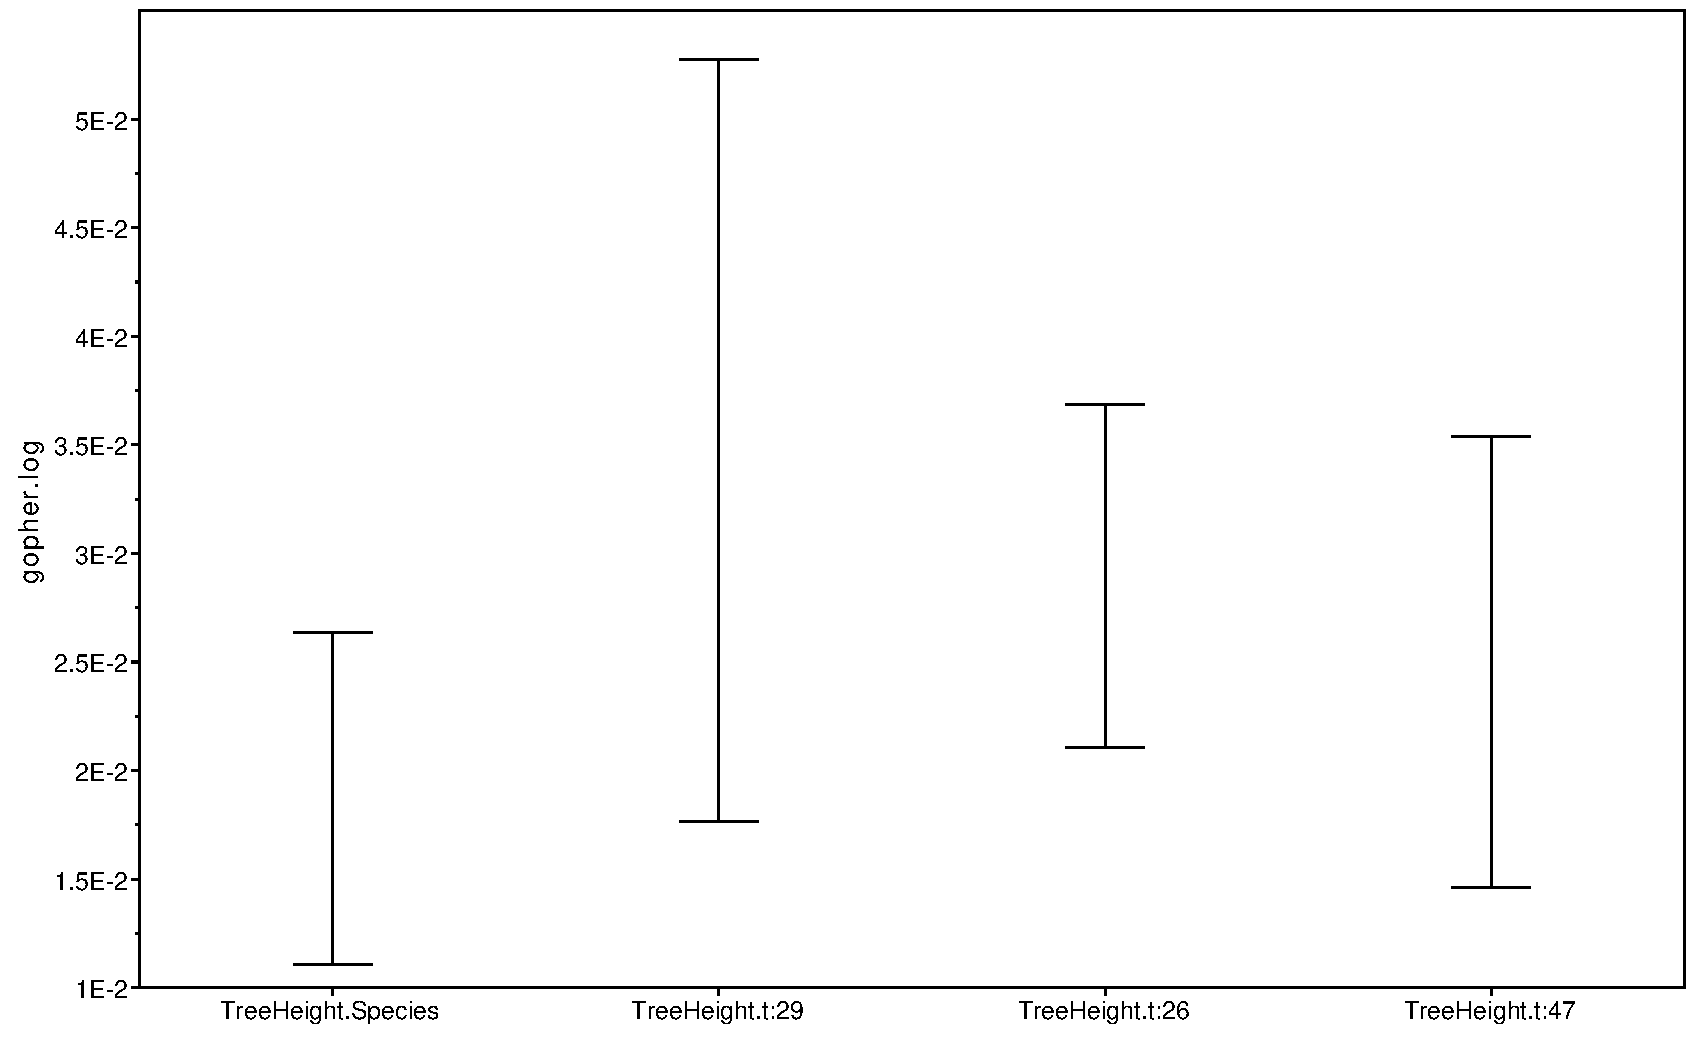
\includegraphics[width=.5\textwidth]{./figures/comp-95HPD.pdf}
%%\caption{The comparison of  95\% HPD intervals from multi-trace}
%%\label{fig:comp95HPD}
%%\end{figure}
%
%%\begin{figure}[H]
%%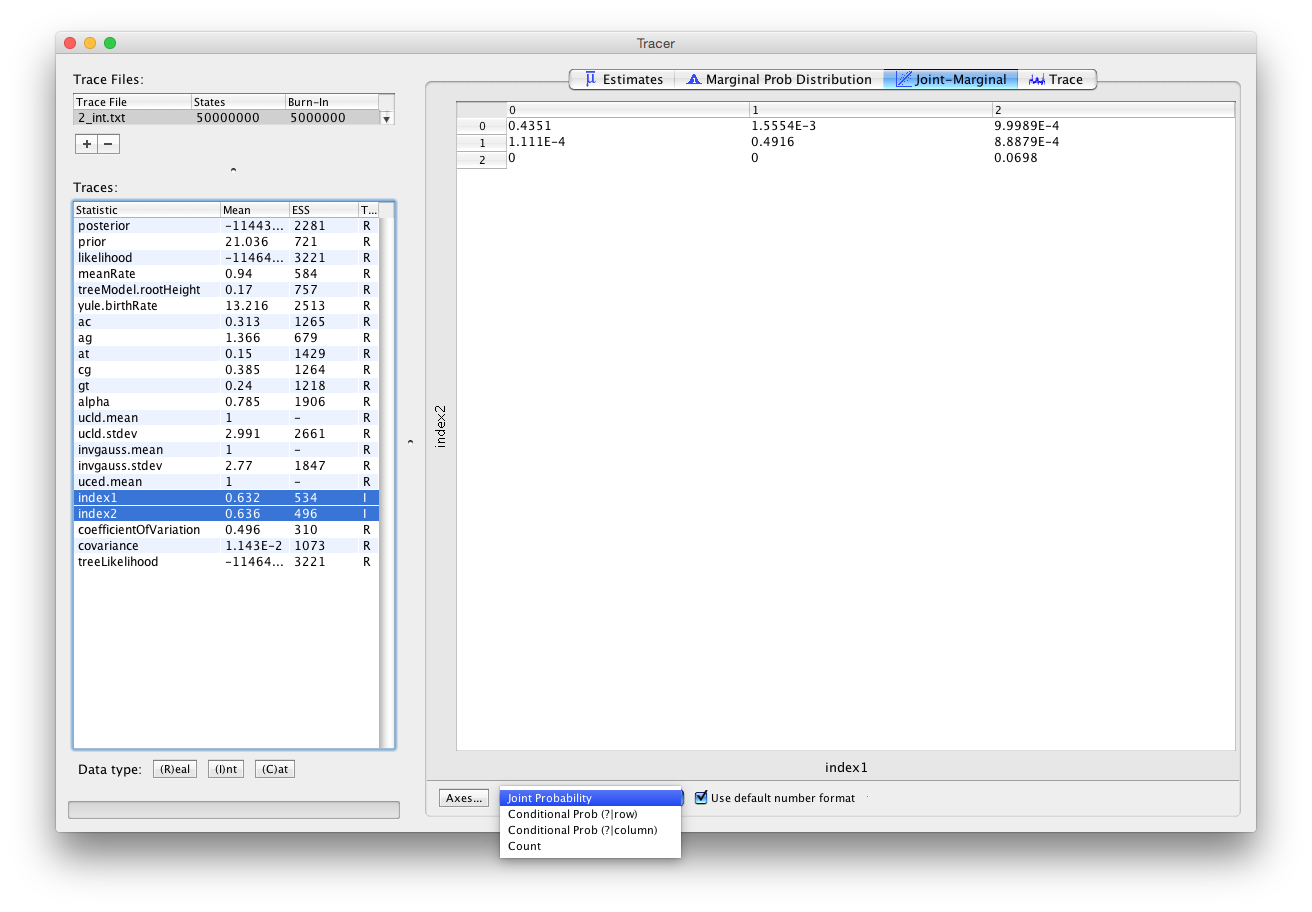
\includegraphics[width=.5\textwidth]{./figures/jointPrInt.png}
%%\caption{The Joint probability table of two integer traces}
%%\label{fig:int:jointpr}
%%\end{figure}
%
%%\begin{figure}[ht]
%%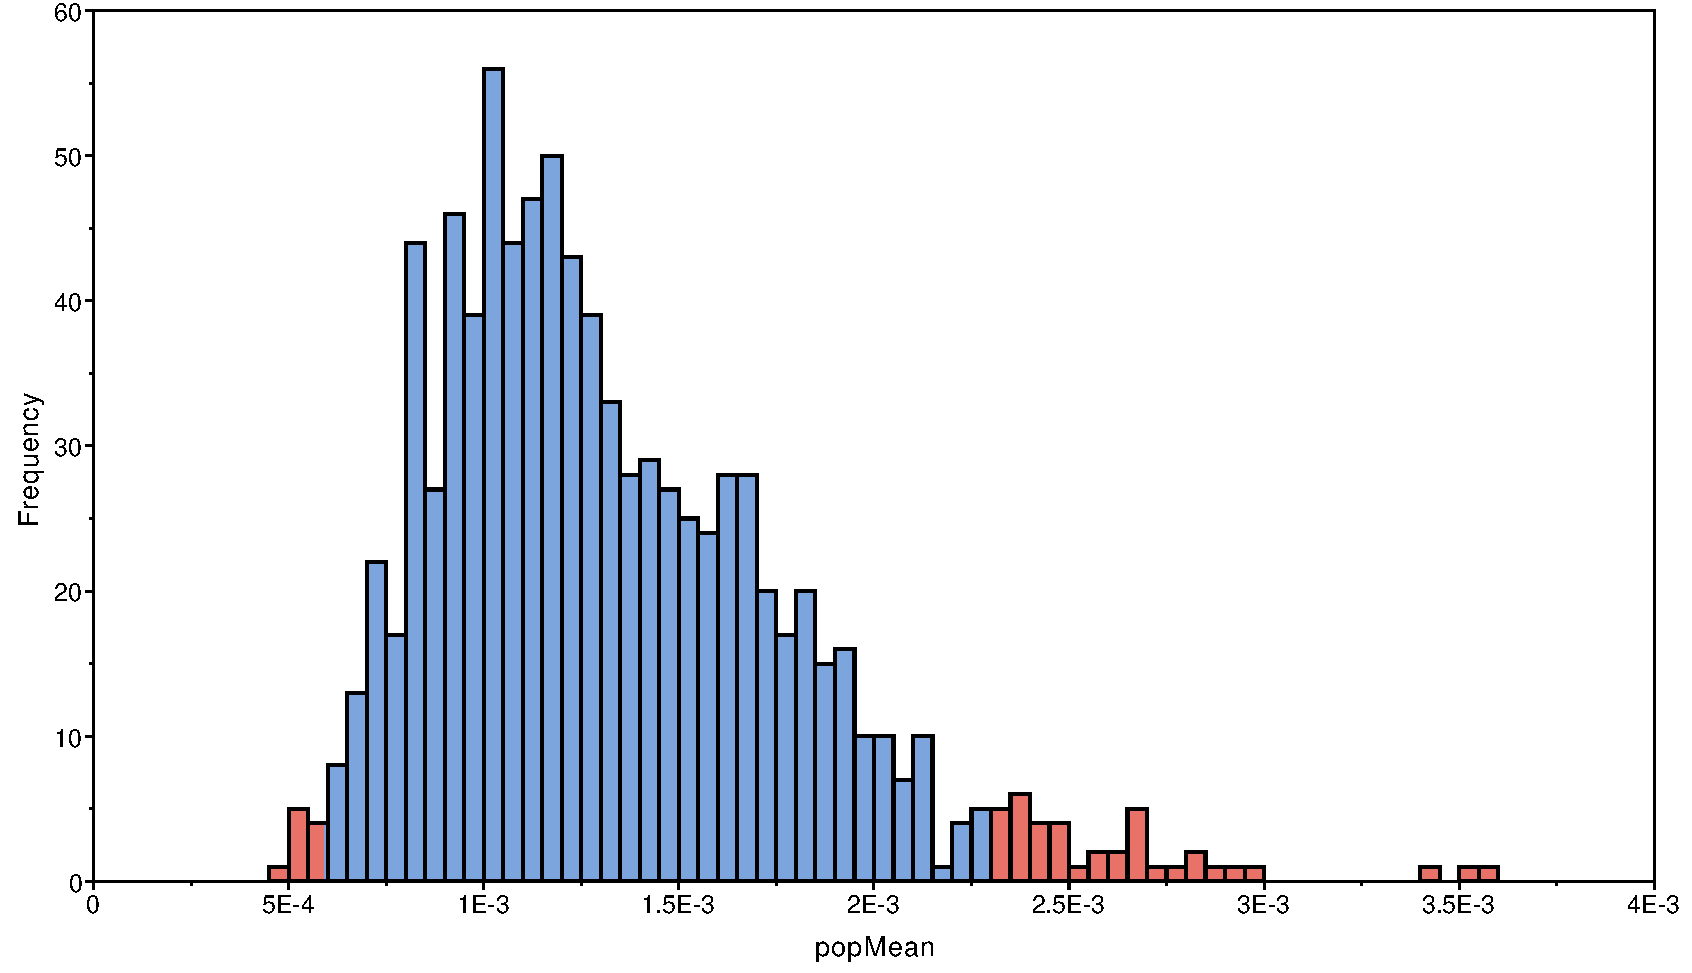
\includegraphics[width=.5\textwidth]{./figures/frequency.pdf}
%%\caption{A frequency distribution for a continuous trace}
%%\label{fig:freq}
%%\end{figure}
%%\begin{figure}[ht]
%%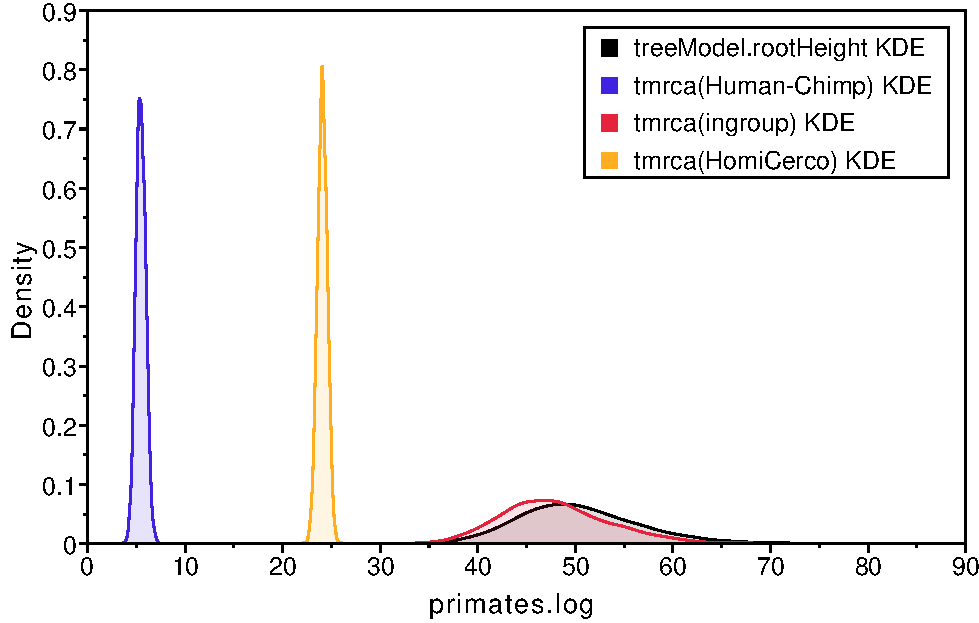
\includegraphics[width=.5\textwidth]{./figures/multiKDE.pdf}
%%\caption{KDE of multiple traces}
%%\label{fig:multiKDE}
%%\end{figure}
%%\begin{figure}[ht]
%%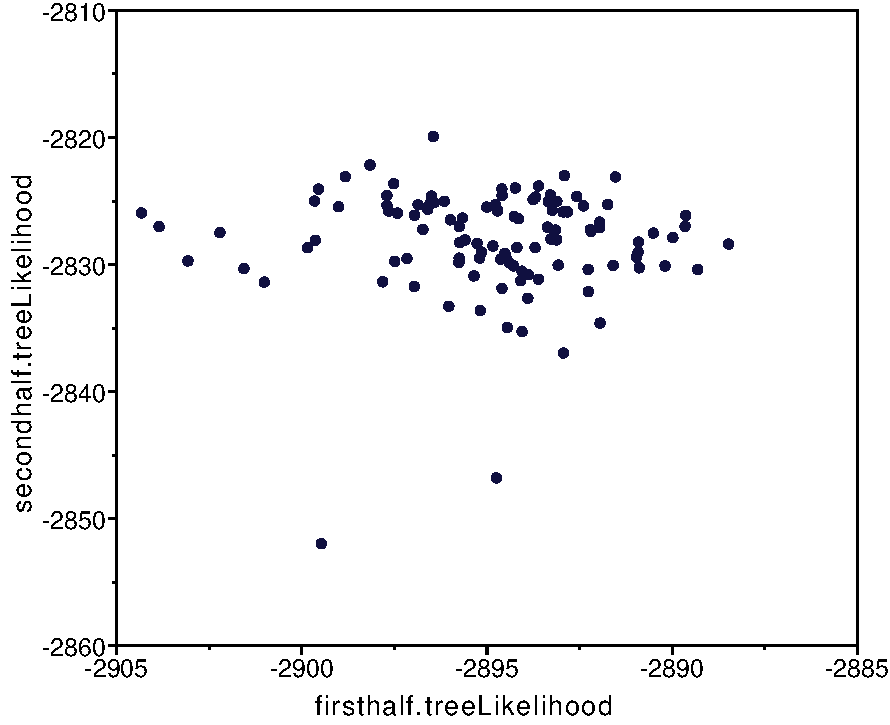
\includegraphics[width=.5\textwidth]{./figures/joint-marginal.pdf}
%%\caption{The joint-marginal distribution of two selected traces}
%%\label{fig:trace}
%%\end{figure}
%%\begin{figure}[ht]
%%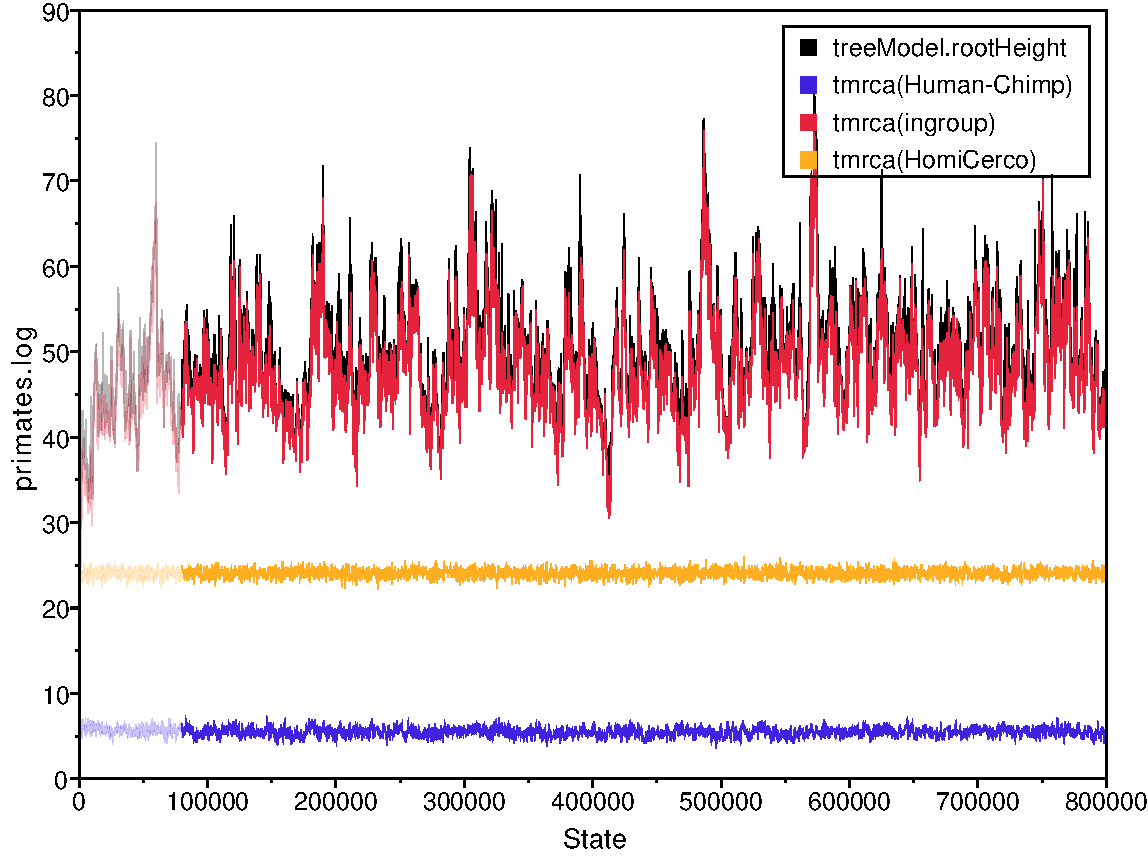
\includegraphics[width=.5\textwidth]{./figures/trace.pdf}
%%\caption{The selected traces against state}
%%\label{fig:trace}
%%\end{figure}
%
%
%\subsubsection*{Diagnostics:} Blah blah
%
%\subsubsection*{Demographic reconstruction:}
%
%%\subsubsection*{Model selection:}
%
%\subsubsection*{Conditional posterior distribution:}

%Fairly general solution to looking at conditional posterior distributions;

%Specifically, support for BSSVS forms of model averaging, in which some parameters are only in the likelihood when their submodel is "indicated" by some indicator function that is usually a discrete, integer or boolean variable. In that case the posterior of the parameter should not include the states when it was sampled only in the prior because the submodel it belonged to was "turned off". This is relevant for EBSP, Random Local Clocks model, microsatellite model averaging and relaxed clock model averaging methods all from my group in last couple of years. Also relevant for BSSVS in phylogeography as well depending on how the state is logged.
%\section*{Taken from the Tracer website}

%Tracer is a program for analysing the trace files generated by Bayesian MCMC runs (that is, the continuous parameter values sampled from the chain). It can be used to analyse runs of BEAST \citep{drummond2012bayesian,drummond2012bayesian}, BEAST2 \citep{bouckaert2014beast2}, MrBayes \citep{ronquist2012mrbayes}, RevBayes \citep{hohna2016revbayes}, LAMARC \citep{kuhner2006lamarc}, Migrate \citep{beerli2006comparison} and possibly other MCMC programs.

%Although Tracer can be used with programs other than BEAST, users may find it useful to join the BEAST users mailing list. This is used to announce new versions and advise users about bugs and problems.

%You can join the mailing list here:
%http://groups.google.com/group/beast-users

%The website for BEAST (and Tracer) is here:
%http://beast.bio.ed.ac.uk/

%At present there is no detailed manual for this application, you will simply have to play around and see what happens. Basically you can select the trace file in the top left of the window, the individual parameter in the bottom left and the analysis appears on the right.

%There are 4 analysis tabs to choose from:

%Estimates - this shows the mean, stdev, confidence intervals and other statistics about the selected parameter. A frequency distribution will also be plotted.
%Density - this shows the Bayesian posterior density plot for the selected parameter.
%Joint-Marginal - this only appears if exactly 2 parameters are chosen (hold down shift to select multiple parameters). It then plots one against the other to look at their joint-marginal distribution.
%Trace - this shows the trace of the parameter against state or generation number. Use this to check mixing, choose a suitable burn-in and look for trends that might suggest problems with convergence.
%Multiple parameters can be selected by holding down the shift key. This will overlay the plots for the different parameters allowing comparisons to be made. You can also select multiple trace files as well to compare different runs. If multiple trace files have the same trace names then a "Combined" trace will automatically appear. This can be selected as well as the individual trace files.

%You can also select the "Demographic Analysis" from the Analysis menu - This plots the distribution of demographic population sizes over time for a number of models (constant size, exponential growth \& logistic growth) that are available in BEAST. This involves you selecting the traces for each parameter of the model. You should only select the model that was actually run under BEAST (e.g., if you ran an exponential growth model, you shouldn't plot the constant population size model).

%The "Analysis" menu also contains options for performing Bayesian Skyline reconstructions and for calculating Bayes Factors between runs.

%The "Print" function in the "File" menu will print the current graph or table and the "Export Data" function can be used to export the data from the plots for use in another graphic package.

%To export the currently displayed graphic use the "Export PDF" function in the "File" menu.


\section*{Acknowledgments}

This work was supported in part by
the Wellcome Trust through project 206298/Z/17/Z (Artic Network),
the European Union Seventh Framework Programme under grant agreement no. 725422-RESERVOIRDOCS,
the National Science Foundation through grant DMS 1264153,
the National Institutes of Health under grant R01 AI107034,
and
the Marsden Trust.

%\section*{References}
% The bibtex filename
\bibliographystyle{natbib}
\bibliography{tracer16}

\end{document}

